%----------------------------------------------------------------------------------------
%	PACKAGES AND THEMES
%----------------------------------------------------------------------------------------
\documentclass[aspectratio=169,xcolor=dvipsnames]{beamer}
\usetheme{Simple}

\usepackage{hyperref}
\usepackage{graphicx} % Allows including images
\usepackage{booktabs} % Allows the use of \toprule, \midrule and \bottomrule in tables
\usepackage{amsmath}

%----------------------------------------------------------------------------------------
%	TITLE PAGE
%----------------------------------------------------------------------------------------

% The title
\title[short title]{Numeric simulation using finite elements}
\subtitle{Sparse but not scarce}

\author {Charlotte Vavourakis, Martin Fasser}
\institute[UIBK] % Your institution may be shorthand to save space
{
    % Your institution for the title page
    University of Innsbruck
    \vskip 3pt
}
\date{\today} % Date, can be changed to a custom date


%----------------------------------------------------------------------------------------
%	PRESENTATION SLIDES
%----------------------------------------------------------------------------------------

\begin{document}

\begin{frame}
    % Print the title page as the first slide
    \titlepage
\end{frame}

%\begin{frame}{Overview}
    % Throughout your presentation, if you choose to use \section{} and \subsection{} commands, these will automatically be printed on this slide as an overview of your presentation
%    \tableofcontents
%\end{frame}

%------------------------------------------------
%\section{First Section}
%------------------------------------------------

%------------------------------------------------
%\section{Second Section}
%------------------------------------------------

\begin{frame}{Original implementation: dense matrix}
    Show recording (or t0/tend) of the solution
\end{frame}

%------------------------------------------------
\begin{frame}{Why Sparse?}
    \begin{columns}[c] % The "c" option specifies centered vertical alignment while the "t" option is used for top vertical alignment

        \column{.45\textwidth} % Left column and width
        
        \textbf{Storage space}
        \begin{center}
    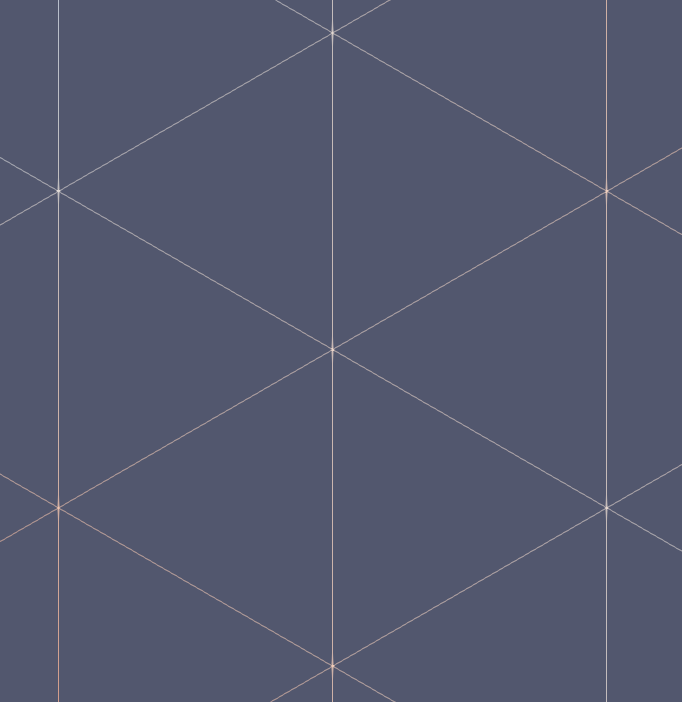
\includegraphics[width=0.3\linewidth]{mesh.png}
    \end{center}
        \begin{enumerate}
        	\item $N=$ number of mesh points
            \item $\approx \; 6 \cdot N $ -nonzero elements in matrix
            \item storage for dense matrix ($\propto N^2$): \\ 2.11 MB
            \item storage for sparse matrix ($\propto N$): \\ 0.05 MB
        \end{enumerate}

        \column{.5\textwidth} % Right column and width
        \begin{center}
    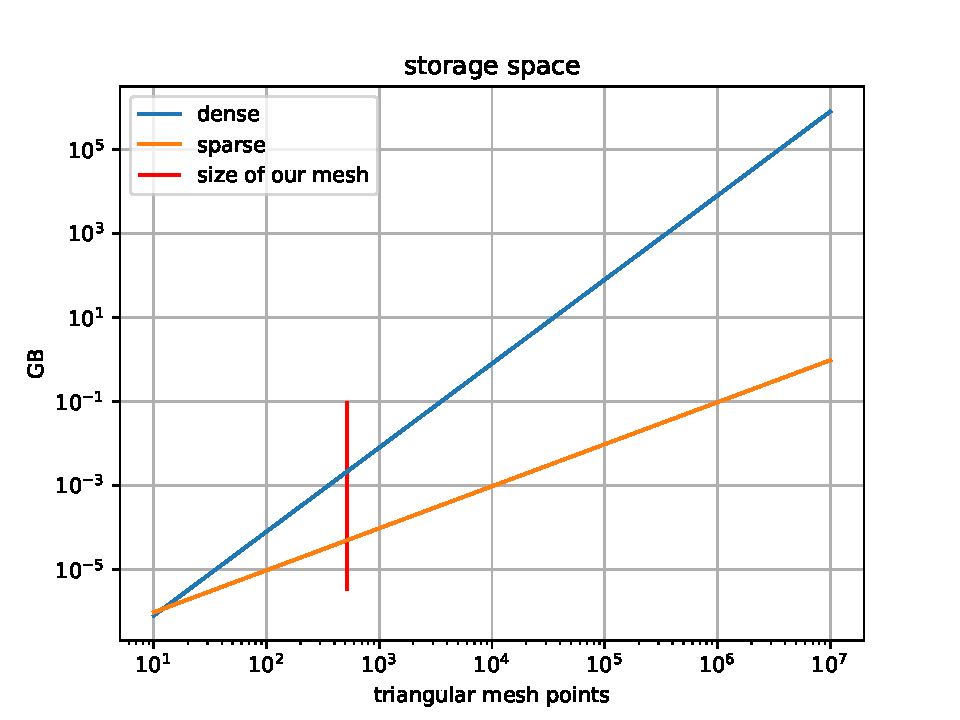
\includegraphics[width=1\linewidth]{storage_space.pdf}
    \end{center}

    \end{columns}
\end{frame}

%------------------------------------------------

\begin{frame}{Assignment: Sparse but not scarce}
	\begin{itemize}
	    \item Convert PDE solver matrix to sparse format and compare the performance with your
	dense matrix implementation.
		\item Use library implementation and compare it with a self-implemented CSR format.

	\end{itemize}
\end{frame}

%------------------------------------------------

\begin{frame}{Solution: Sparse but not scarce}
	\begin{itemize}
		\item two self-implemented classes for sparse matrices: non-CSR and CSR format.
	\end{itemize}
	
\centerline{Explain a little?}

	\begin{itemize}
		\item Eigen library:
	\end{itemize}
	
\centerline{SparseMatrix class, with SparseMatrix::makeCompressed() conversion to CSR} 

	\begin{itemize}
		\item Bonus, Forward Euler written using matrix multiplication: 
	\end{itemize}
	
 \centerline{SparseMatrix B * VectorXd u} 
    
	
\end{frame}

%------------------------------------------------
\begin{frame}{Different Sparse Formats}
    \begin{columns}[c] % The "c" option specifies centered vertical alignment while the "t" option is used for top vertical alignment

\column{.65\textwidth} % Left column and width
\begin{itemize}
\item sparse - manual
  \begin{itemize}
     	\item $\mathrm{values} =  \begin{bmatrix} 
		5.3, & 1.5, & 4.2, & 3.1, & 2, & 2.2, & 1.9 
		\end{bmatrix}$

		\item $\mathrm{pos} = \begin{bmatrix}
		1, & 4, & 5, & 7, & 9, & 18, & 20 
		\end{bmatrix}$
	\end{itemize}
\item sparse - coo (coordinate list)
	\begin{itemize}
		\item $\mathrm{values} = \begin{bmatrix}
		5.3, & 1.5, & 4.2, & 3.1, & 2, & 2.2, & 1.9 
		\end{bmatrix}$
		\item $\mathrm{col\_ind} = \begin{bmatrix}
		1, & 4, & 0, & 2, & 4, & 3, & 0 
		\end{bmatrix}$
		\item $\mathrm{row\_ind} = \begin{bmatrix}
		0, & 0, & 1, & 1, & 1, & 3, & 4 
		\end{bmatrix}$
	\end{itemize}
\item sparse - csr (compressed row storage)
	\begin{itemize}
       \item $\mathrm{values} = \begin{bmatrix}
		5.3, & 1.5, & 4.2, & 3.1, & 2, & 2.2, & 1.9 
		\end{bmatrix}$
		\item $\mathrm{col\_ind} = \begin{bmatrix}
		1, & 4, & 0, & 2, & 4, & 3, & 0 
		\end{bmatrix}$
		\item $\mathrm{row\_ptr} = \begin{bmatrix}
		0, & 2, & 5, & 5, & 6, & 7 
		\end{bmatrix}$
	\end{itemize}
\end{itemize}
        
        \column{.3\textwidth} % Right column and width
        $ \left( \begin{array}{rrrrr} 
0 & 5.3 & 0 & 0 & 1.5\\ 
4.2 & 0& 3.1 & 0 & 2\\ 
0 & 0 & 0 & 0 & 0 \\
0 & 0 & 0 & 2.2 & 0 \\
1.9 & 0 & 0 & 0 & 0
\end{array} \right) $

    \end{columns}
\end{frame}

%------------------------------------------------
\begin{frame}{Matrix assembly}

\end{frame}
%------------------------------------------------
\begin{frame}{Conversion coo to csr}
    \begin{columns}[c] % The "c" option specifies centered vertical alignment while the "t" option is used for top vertical alignment

\column{.65\textwidth} % Left column and width
coo format: \\
$\mathrm{row\_ind} = \begin{bmatrix}
		0, & 0, & 1, & 1, & 1, & 3, & 4 
		\end{bmatrix}$

\begin{center}
    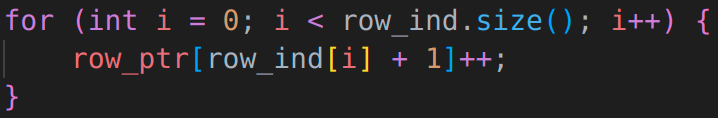
\includegraphics[width=0.7\linewidth]{conversion1.png}
    \end{center}

how many elements in each row:
$\mathrm{row\_step} = \begin{bmatrix}
		0, & 2, & 3, & 0, & 1, & 1 
		\end{bmatrix}$

\begin{center}
    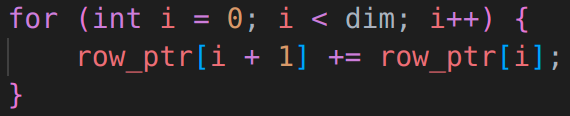
\includegraphics[width=0.7\linewidth]{conversion2.png}
    \end{center}

csr format: \\
$\mathrm{row\_ptr} = \begin{bmatrix}
		0, & 2, & 5, & 5, & 6, & 7 
		\end{bmatrix}$

        
\column{.3\textwidth} % Right column and width
        $ \left( \begin{array}{rrrrr} 
0 & 5.3 & 0 & 0 & 1.5\\ 
4.2 & 0& 3.1 & 0 & 2\\ 
0 & 0 & 0 & 0 & 0 \\
0 & 0 & 0 & 2.2 & 0 \\
1.9 & 0 & 0 & 0 & 0
\end{array} \right) $

    \end{columns}
\end{frame}

%------------------------------------------------

\begin{frame}{Sparse - manual}
    \begin{columns}[c] % The "c" option specifies centered vertical alignment while the "t" option is used for top vertical alignment

\column{.65\textwidth} % Left column and width
\begin{itemize}
\item sparse - manual
  \begin{itemize}
     	\item $\mathrm{values} =  \begin{bmatrix} 
		5.3, & 1.5, & 4.2, & 3.1, & 2, & 2.2, & 1.9 
		\end{bmatrix}$

		\item $\mathrm{pos} = \begin{bmatrix}
		1, & 4, & 5, & 7, & 9, & 18, & 20 
		\end{bmatrix}$
	\end{itemize}
\item matrix-vector multiplication
\begin{center}
    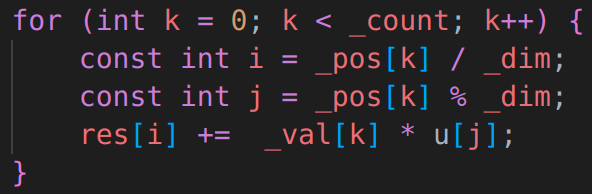
\includegraphics[width=0.8\linewidth]{matrix_vector_man2.png}
    \end{center}
\end{itemize}

        
        \column{.3\textwidth} % Right column and width
        $ \left( \begin{array}{rrrrr} 
0 & 5.3 & 0 & 0 & 1.5\\ 
4.2 & 0& 3.1 & 0 & 2\\ 
0 & 0 & 0 & 0 & 0 \\
0 & 0 & 0 & 2.2 & 0 \\
1.9 & 0 & 0 & 0 & 0
\end{array} \right) $

    \end{columns}
\end{frame}

%------------------------------------------------

\begin{frame}{Sparse - CSR}
    \begin{columns}[c] % The "c" option specifies centered vertical alignment while the "t" option is used for top vertical alignment

\column{.65\textwidth} % Left column and width
\begin{itemize}
\item sparse - csr (compressed row storage)
	\begin{itemize}
       \item $\mathrm{values} = \begin{bmatrix}
		5.3, & 1.5, & 4.2, & 3.1, & 2, & 2.2, & 1.9 
		\end{bmatrix}$
		\item $\mathrm{col\_ind} = \begin{bmatrix}
		1, & 4, & 0, & 2, & 4, & 3, & 0 
		\end{bmatrix}$
		\item $\mathrm{row\_ptr} = \begin{bmatrix}
		0, & 2, & 5, & 5, & 6, & 7 
		\end{bmatrix}$
	\end{itemize}
\item matrix-vector multiplication
\begin{center}
    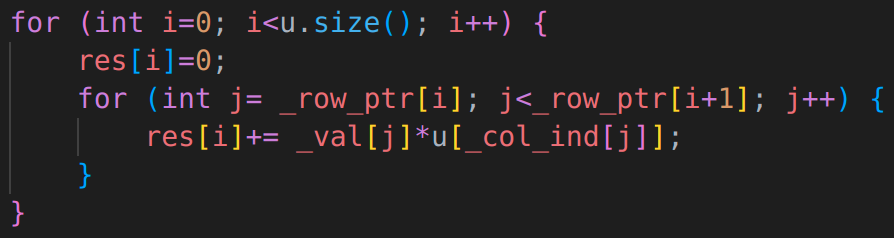
\includegraphics[width=0.8\linewidth]{matrix_vector_csr.png}
    \end{center}
\end{itemize}
        
        \column{.3\textwidth} % Right column and width
        $ \left( \begin{array}{rrrrr} 
0 & 5.3 & 0 & 0 & 1.5\\ 
4.2 & 0& 3.1 & 0 & 2\\ 
0 & 0 & 0 & 0 & 0 \\
0 & 0 & 0 & 2.2 & 0 \\
1.9 & 0 & 0 & 0 & 0
\end{array} \right) $

    \end{columns}
\end{frame}

%------------------------------------------------

\begin{frame}{Google Benchmark}
    \begin{itemize}
        \item github.com/google/benchmark
        \item a library to benchmark code snippets (functions) 
        \item added to to repository as a git submodule
    \end{itemize}
    
    \begin{center}
    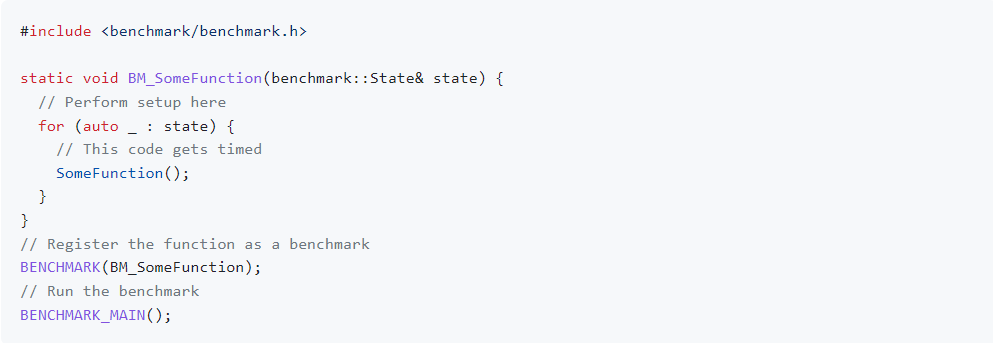
\includegraphics[width=0.8\linewidth]{example_google_benchmark.png}
    \end{center}
\end{frame}

%------------------------------------------------

\begin{frame}{Code organization}
    \begin{itemize}
        \item Cmake build 8 targets, common + unique code
        \item 4 versions of PDE solver
        \item corresponding benchmarks, testing functions unique to each implementation 
    \end{itemize}
    
    \begin{center}
    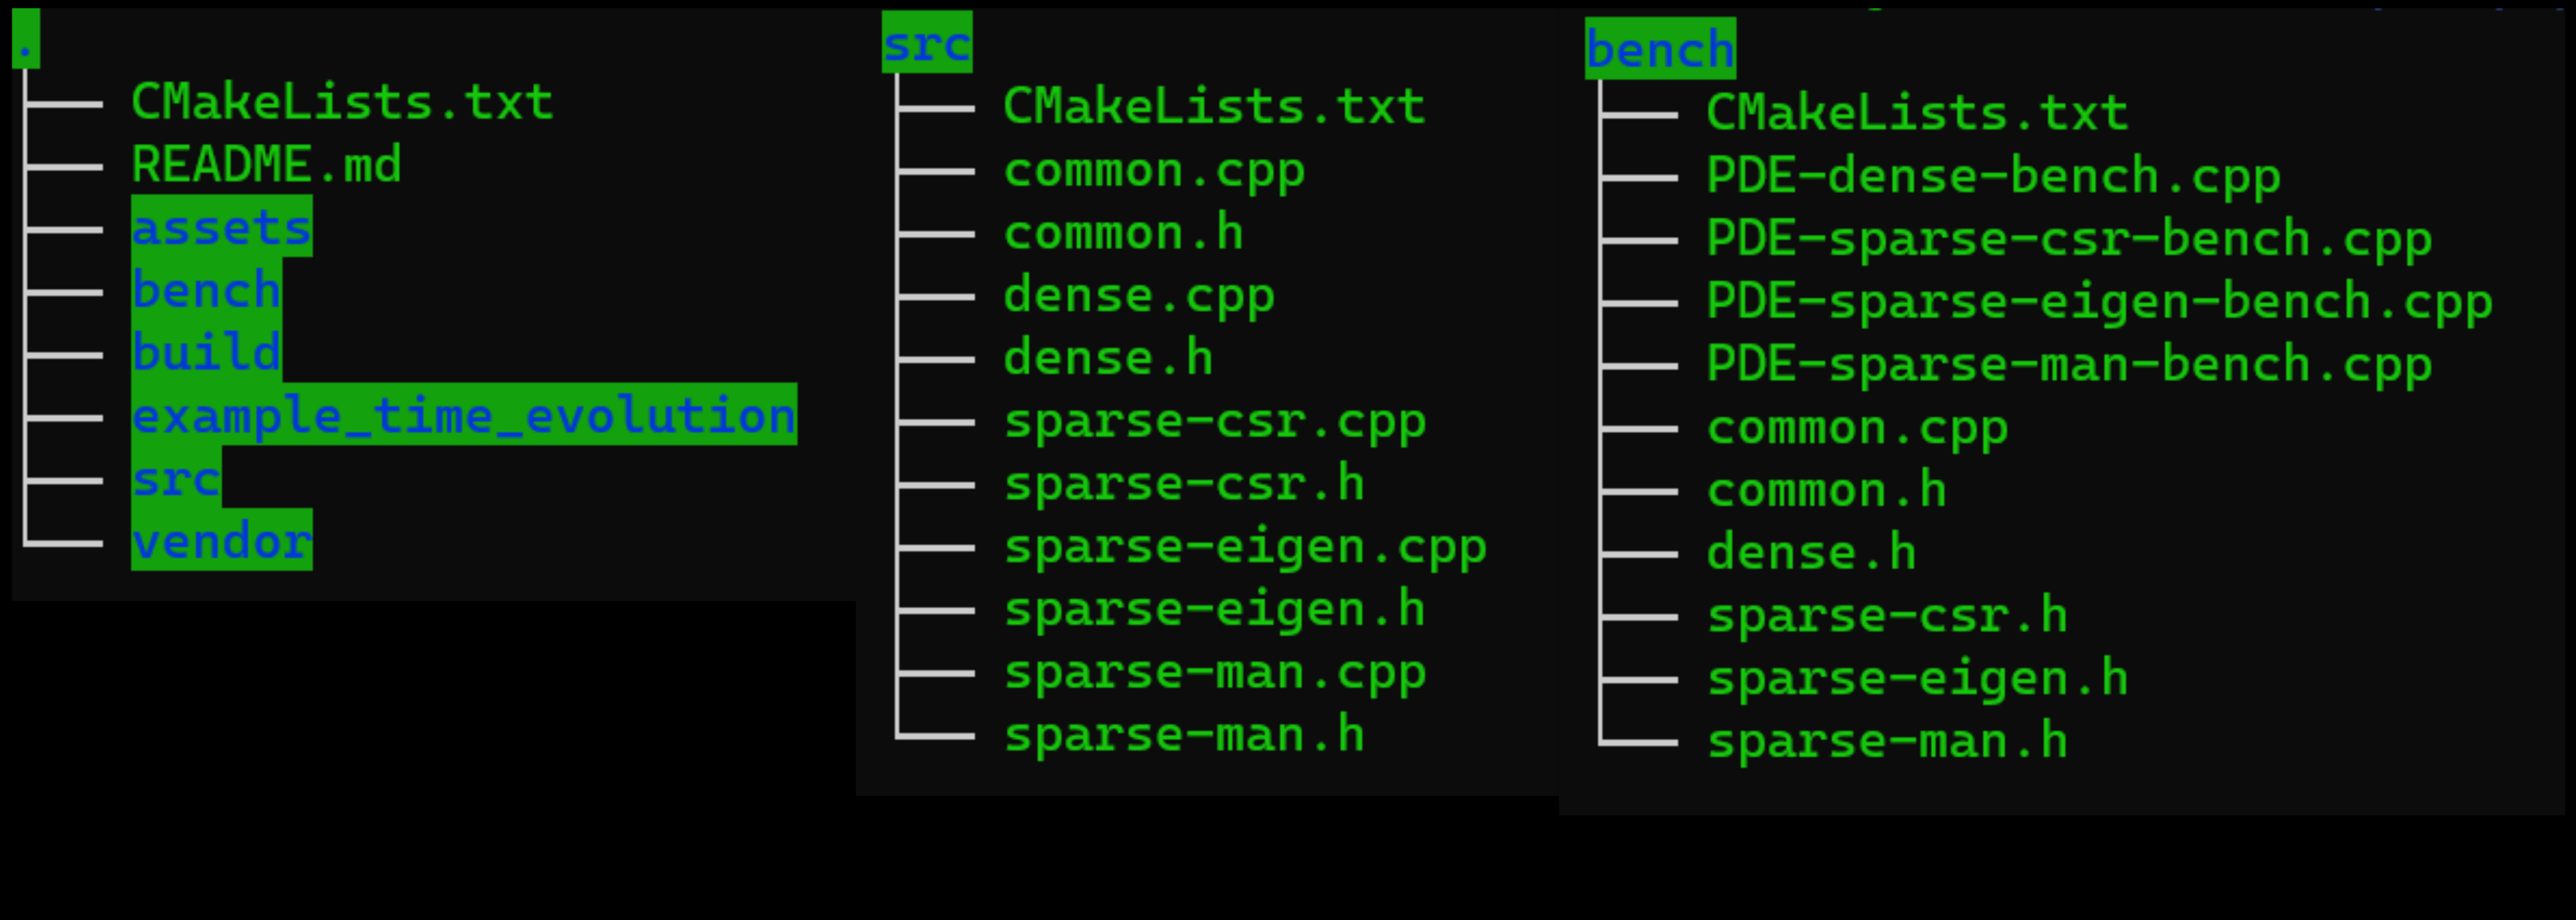
\includegraphics[width=0.8\linewidth]{code_structure.png}
    \end{center}
\end{frame}

%------------------------------------------------

\begin{frame}{Benchmark assembly matrix B}
   
   Example output
   
\end{frame}

%------------------------------------------------

\begin{frame}{Benchmark assembly matrix B}
   
   Graph or table comparing 4 implementations
   
\end{frame}

%------------------------------------------------

\begin{frame}{Benchmark time evolution}
   
   Graph or table comparing 4 implementations
   
\end{frame}

%------------------------------------------------

\begin{frame}{Benchmark assembly B + time evolution for different dt }
   
   Graph or table comparing 4 implementations
   
\end{frame}

%------------------------------------------------

\begin{frame}{Conclusions}
   \begin{itemize}
	  \item Using the sparse format for B resulted in a 10-fold time speed up
	  \item With Eigen even more speed up and code simplification using matrix product expressions
   \end{itemize}
\end{frame}

%------------------------------------------------

\begin{frame}
    \Huge{\centerline{Questions?}}
\end{frame}

%----------------------------------------------------------------------------------------

\begin{frame}{Blocks of Highlighted Text}
    In this slide, some important text will be \alert{highlighted} because it's important. Please, don't abuse it.

    \begin{block}{Block}
        Sample text
    \end{block}

    \begin{alertblock}{Alertblock}
        Sample text in red box
    \end{alertblock}

    \begin{examples}
        Sample text in green box. The title of the block is ``Examples".
    \end{examples}
\end{frame}

%------------------------------------------------

\begin{frame}{Multiple Columns}
    \begin{columns}[c] % The "c" option specifies centered vertical alignment while the "t" option is used for top vertical alignment

        \column{.45\textwidth} % Left column and width
        \textbf{Heading}
        \begin{enumerate}
            \item Statement
            \item Explanation
            \item Example
        \end{enumerate}

        \column{.5\textwidth} % Right column and width
        Lorem ipsum dolor sit amet, consectetur adipiscing elit. Integer lectus nisl, ultricies in feugiat rutrum, porttitor sit amet augue. Aliquam ut tortor mauris. Sed volutpat ante purus, quis accumsan dolor.

    \end{columns}
\end{frame}

%------------------------------------------------

\begin{frame}{Table}
    \begin{table}
        \begin{tabular}{l l l}
            \toprule
            \textbf{Treatments} & \textbf{Response 1} & \textbf{Response 2} \\
            \midrule
            Treatment 1         & 0.0003262           & 0.562               \\
            Treatment 2         & 0.0015681           & 0.910               \\
            Treatment 3         & 0.0009271           & 0.296               \\
            \bottomrule
        \end{tabular}
        \caption{Table caption}
    \end{table}
\end{frame}

%------------------------------------------------

\begin{frame}{Theorem}
    \begin{theorem}[Mass--energy equivalence]
        $E = mc^2$
    \end{theorem}
\end{frame}

%------------------------------------------------

\begin{frame}{Figure}
    Uncomment the code on this slide to include your own image from the same directory as the template .TeX file.
    %\begin{figure}
    %\includegraphics[width=0.8\linewidth]{test}
    %\end{figure}
\end{frame}

%------------------------------------------------

\begin{frame}[fragile] % Need to use the fragile option when verbatim is used in the slide
    \frametitle{Citation}
    An example of the \verb|\cite| command to cite within the presentation:\\~

    This statement requires citation \cite{p1}.
\end{frame}

%------------------------------------------------

\begin{frame}{References}
    % Beamer does not support BibTeX so references must be inserted manually as below
    \footnotesize{
        \begin{thebibliography}{99}
            \bibitem[Smith, 2012]{p1} John Smith (2012)
            \newblock Title of the publication
            \newblock \emph{Journal Name} 12(3), 45 -- 678.
        \end{thebibliography}
    }
\end{frame}

%------------------------------------------------

\end{document}